% $Id: template.tex 11 2007-04-03 22:25:53Z jpeltier $

\documentclass{vgtc}                          % final (conference style)
%\documentclass[review]{vgtc}                 % review
%\documentclass[widereview]{vgtc}             % wide-spaced review
%\documentclass[preprint]{vgtc}               % preprint
%\documentclass[electronic]{vgtc}             % electronic version

%% Uncomment one of the lines above depending on where your paper is
%% in the conference process. ``review'' and ``widereview'' are for review
%% submission, ``preprint'' is for pre-publication, and the final version
%% doesn't use a specific qualifier. Further, ``electronic'' includes
%% hyperreferences for more convenient online viewing.

%% Please use one of the ``review'' options in combination with the
%% assigned online id (see below) ONLY if your paper uses a double blind
%% review process. Some conferences, like IEEE Vis and InfoVis, have NOT
%% in the past.

%% Figures should be in CMYK or Grey scale format, otherwise, colour 
%% shifting may occur during the printing process.

%% These few lines make a distinction between latex and pdflatex calls and they
%% bring in essential packages for graphics and font handling.
%% Note that due to the \DeclareGraphicsExtensions{} call it is no longer necessary
%% to provide the the path and extension of a graphics file:
%% \includegraphics{diamondrule} is completely sufficient.
%%
\ifpdf%                                % if we use pdflatex
  \pdfoutput=1\relax                   % create PDFs from pdfLaTeX
  \pdfcompresslevel=9                  % PDF Compression
  \pdfoptionpdfminorversion=7          % create PDF 1.7
  \ExecuteOptions{pdftex}
  \usepackage{graphicx}                % allow us to embed graphics files
  \DeclareGraphicsExtensions{.pdf,.png,.jpg,.jpeg} % for pdflatex we expect .pdf, .png, or .jpg files
\else%                                 % else we use pure latex
  \ExecuteOptions{dvips}
  \usepackage{graphicx}                % allow us to embed graphics files
  \DeclareGraphicsExtensions{.eps}     % for pure latex we expect eps files
\fi%

%% it is recomended to use ``\autoref{sec:bla}'' instead of ``Fig.~\ref{sec:bla}''
\graphicspath{{figures/}{pictures/}{images/}{./}} % where to search for the images

\usepackage{microtype}                 % use micro-typography (slightly more compact, better to read)
\PassOptionsToPackage{warn}{textcomp}  % to address font issues with \textrightarrow
\usepackage{textcomp}                  % use better special symbols
\usepackage{mathptmx}                  % use matching math font
\usepackage{times}                     % we use Times as the main font
\renewcommand*\ttdefault{txtt}         % a nicer typewriter font
\usepackage{cite}                      % needed to automatically sort the references
\usepackage{tabu}                      % only used for the table example
\usepackage{booktabs}                  % only used for the table example
%% We encourage the use of mathptmx for consistent usage of times font
%% throughout the proceedings. However, if you encounter conflicts
%% with other math-related packages, you may want to disable it.


%% If you are submitting a paper to a conference for review with a double
%% blind reviewing process, please replace the value ``0'' below with your
%% OnlineID. Otherwise, you may safely leave it at ``0''.
\onlineid{0}

%% declare the category of your paper, only shown in review mode
\vgtccategory{Research}

%% allow for this line if you want the electronic option to work properly
\vgtcinsertpkg

%% In preprint mode you may define your own headline.
%\preprinttext{To appear in an IEEE VGTC sponsored conference.}

%% Paper title.

\title{DigiDrum}

%% This is how authors are specified in the conference style

%% Author and Affiliation (single author).
%%\author{Roy G. Biv\thanks{e-mail: roy.g.biv@aol.com}}
%%\affiliation{\scriptsize Allied Widgets Research}

%% Author and Affiliation (multiple authors with single affiliations).
%%\author{Roy G. Biv\thanks{e-mail: roy.g.biv@aol.com} %
%%\and Ed Grimley\thanks{e-mail:ed.grimley@aol.com} %
%%\and Martha Stewart\thanks{e-mail:martha.stewart@marthastewart.com}}
%%\affiliation{\scriptsize Martha Stewart Enterprises \\ Microsoft Research}

%% Author and Affiliation (multiple authors with multiple affiliations)
\author{Silvin Willemsen\thanks{e-mail: roy.g.biv@aol.com}\\ %
        \scriptsize Aalborg University \\ Multisensory Experience Lab %
\and Mauro Nascimben\thanks{e-mail: ed.grimley@aol.com}\\ %
     \scriptsize Aalborg University %
\and Anca-Simona Horvath\thanks{e-mail: ancah@hum.aau.dk}\\ %
     \parbox{1.4in}{\scriptsize \centering Aalborg University\\Research Laboratory in Art&Technology}}

%% A teaser figure can be included as follows, but is not recommended since
%% the space is now taken up by a full width abstract.
%\teaser{
%  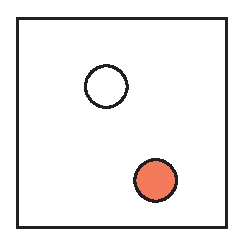
\includegraphics[width=1.5in]{sample.eps}
%  \caption{Lookit! Lookit!}
%}

%% Abstract section.
\abstract{DigiDrum is a Virtual Reality musical instrument. We Lorem ipsum dolor sit amet, consectetuer adipiscing elit,
sed diam nonummy nibh euismod tincidunt ut laoreet dolore magna
aliquam erat volutpat. Ut wisi enim ad minim veniam, quis nostrud exerci tation ullamcorper
suscipit lobortis nisl ut aliquip ex ea commodo consequat. Duis autem
vel eum iriure dolor in hendrerit in vulputate velit esse molestie
consequat, vel illum dolore eu feugiat nulla facilisis at vero eros et
accumsan et iusto odio dignissim qui blandit praesent luptatum zzril
delenit augue duis dolore te feugait nulla facilisi.%
} % end of abstract

%% ACM Computing Classification System (CCS). 
%% See <http://www.acm.org/about/class> for details.
%% We recommend the 2012 system <http://www.acm.org/about/class/class/2012>
%% For the 2012 system use the ``\CCScatTwelve'' which command takes four arguments.
%% The 1998 system <http://www.acm.org/about/class/class/2012> is still possible
%% For the 1998 system use the ``\CCScat'' which command takes four arguments.
%% In both cases the last two arguments (1998) or last three (2012) can be empty.

\CCScatlist{
  \CCScatTwelve{Human-centered computing}{Visu\-al\-iza\-tion}{Visu\-al\-iza\-tion techniques}{Treemaps};
  \CCScatTwelve{Human-centered computing}{Visu\-al\-iza\-tion}{Visualization design and evaluation methods}{}
}

%\CCScatlist{
  %\CCScat{H.5.2}{User Interfaces}{User Interfaces}{Graphical user interfaces (GUI)}{};
  %\CCScat{H.5.m}{Information Interfaces and Presentation}{Miscellaneous}{}{}
%}

%% Copyright space is enabled by default as required by guidelines.
%% It is disabled by the 'review' option or via the following command:
% \nocopyrightspace

%%%%%%%%%%%%%%%%%%%%%%%%%%%%%%%%%%%%%%%%%%%%%%%%%%%%%%%%%%%%%%%%
%%%%%%%%%%%%%%%%%%%%%% START OF THE PAPER %%%%%%%%%%%%%%%%%%%%%%
%%%%%%%%%%%%%%%%%%%%%%%%%%%%%%%%%%%%%%%%%%%%%%%%%%%%%%%%%%%%%%%%%

\begin{document}

%% The ``\maketitle'' command must be the first command after the
%% ``\begin{document}'' command. It prepares and prints the title block.

%% the only exception to this rule is the \firstsection command
\firstsection{Introduction}

\maketitle

%% \section{Introduction} %for journal use above \firstsection{..} instead
This template is for papers of VGTC-sponsored conferences which are \emph{\textbf{not}} published in a special issue of TVCG.

\section{Using the Style Template}

\begin{itemize}
\item If you receive compilation errors along the lines of ``\texttt{Package ifpdf Error: Name clash, \textbackslash ifpdf is already defined}'' then please add a new line ``\texttt{\textbackslash let\textbackslash ifpdf\textbackslash relax}'' right after the ``\texttt{\textbackslash documentclass[journal]\{vgtc\}}'' call. Note that your error is due to packages you use that define ``\texttt{\textbackslash ifpdf}'' which is obsolete (the result is that \texttt{\textbackslash ifpdf} is defined twice); these packages should be changed to use ifpdf package instead.
\item The style uses the hyperref package, thus turns references into internal links. We thus recommend to make use of the ``\texttt{\textbackslash autoref\{reference\}}'' call (instead of ``\texttt{Figure\~{}\textbackslash ref\{reference\}}'' or similar) since ``\texttt{\textbackslash autoref\{reference\}}'' turns the entire reference into an internal link, not just the number. Examples: \autoref{fig:sample} and \autoref{tab:vis_papers}.
\item The style automatically looks for image files with the correct extension (eps for regular \LaTeX; pdf, png, and jpg for pdf\LaTeX), in a set of given subfolders (figures/, pictures/, images/). It is thus sufficient to use ``\texttt{\textbackslash includegraphics\{CypressView\}}'' (instead of ``\texttt{\textbackslash includegraphics\{pictures/CypressView.jpg\}}'').
\item For adding hyperlinks and DOIs to the list of references, you can use ``\texttt{\textbackslash bibliographystyle\{abbrv-doi-hyperref-narrow\}}'' (instead of ``\texttt{\textbackslash bibliographystyle\{abbrv\}}''). It uses the doi and url fields in a bib\TeX\ entry and turns the entire reference into a link, giving priority to the doi. The doi can be entered with or without the ``\texttt{http://dx.doi.org/}'' url part. See the examples in the bib\TeX\ file and the bibliography at the end of this template.\\[1em]
\textbf{Note 1:} occasionally (for some \LaTeX\ distributions) this hyper-linked bib\TeX\ style may lead to \textbf{compilation errors} (``\texttt{pdfendlink ended up in different nesting level ...}'') if a reference entry is broken across two pages (due to a bug in hyperref). In this case make sure you have the latest version of the hyperref package (i.\,e., update your \LaTeX\ installation/packages) or, alternatively, revert back to ``\texttt{\textbackslash bibliographystyle\{abbrv-doi-narrow\}}'' (at the expense of removing hyperlinks from the bibliography) and try ``\texttt{\textbackslash bibliographystyle\{abbrv-doi-hyperref-narrow\}}'' again after some more editing.\\[1em]
\textbf{Note 2:} the ``\texttt{-narrow}'' versions of the bibliography style use the font ``PTSansNarrow-TLF'' for typesetting the DOIs in a compact way. This font needs to be available on your \LaTeX\ system. It is part of the \href{https://www.ctan.org/pkg/paratype}{``paratype'' package}, and many distributions (such as MikTeX) have it automatically installed. If you do not have this package yet and want to use a ``\texttt{-narrow}'' bibliography style then use your \LaTeX\ system's package installer to add it. If this is not possible you can also revert to the respective bibliography styles without the ``\texttt{-narrow}'' in the file name.\\[1em]
DVI-based processes to compile the template apparently cannot handle the different font so, by default, the template file uses the \texttt{abbrv-doi} bibliography style but the compiled PDF shows you the effect of the \texttt{abbrv-doi-hyperref-narrow} style.
\end{itemize}

\section{Bibliography Instructions}

\begin{itemize}
\item Sort all bibliographic entries alphabetically but the last name of the first author. This \LaTeX/bib\TeX\ template takes care of this sorting automatically.
\item Merge multiple references into one; e.\,g., use \cite{Max:1995:OMF,Kitware:2003} (not \cite{Kitware:2003}\cite{Max:1995:OMF}). Within each set of multiple references, the references should be sorted in ascending order. This \LaTeX/bib\TeX\ template takes care of both the merging and the sorting automatically.
\item Verify all data obtained from digital libraries, even ACM's DL and IEEE Xplore  etc.\ are sometimes wrong or incomplete.
\item Do not trust bibliographic data from other services such as Mendeley.com, Google Scholar, or similar; these are even more likely to be incorrect or incomplete.
\item Articles in journal---items to include:
  \begin{itemize}
  \item author names
	\item title
	\item journal name
	\item year
	\item volume
	\item number
	\item month of publication as variable name (i.\,e., \{jan\} for January, etc.; month ranges using \{jan \#\{/\}\# feb\} or \{jan \#\{-{}-\}\# feb\})
  \end{itemize}
\item use journal names in proper style: correct: ``IEEE Transactions on Visualization and Computer Graphics'', incorrect: ``Visualization and Computer Graphics, IEEE Transactions on''
\item Papers in proceedings---items to include:
  \begin{itemize}
  \item author names
	\item title
	\item abbreviated proceedings name: e.\,g., ``Proc.\textbackslash{} CONF\_ACRONYNM'' without the year; example: ``Proc.\textbackslash{} CHI'', ``Proc.\textbackslash{} 3DUI'', ``Proc.\textbackslash{} Eurographics'', ``Proc.\textbackslash{} EuroVis''
	\item year
	\item publisher
	\item town with country of publisher (the town can be abbreviated for well-known towns such as New York or Berlin)
  \end{itemize}
\item article/paper title convention: refrain from using curly brackets, except for acronyms/proper names/words following dashes/question marks etc.; example:
\begin{itemize}
	\item paper ``Marching Cubes: A High Resolution 3D Surface Construction Algorithm''
	\item should be entered as ``\{M\}arching \{C\}ubes: A High Resolution \{3D\} Surface Construction Algorithm'' or  ``\{M\}arching \{C\}ubes: A high resolution \{3D\} surface construction algorithm''
	\item will be typeset as ``Marching Cubes: A high resolution 3D surface construction algorithm''
\end{itemize}
\item for all entries
\begin{itemize}
	\item DOI can be entered in the DOI field as plain DOI number or as DOI url; alternative: a url in the URL field
	\item provide full page ranges AA-{}-BB
\end{itemize}
\item when citing references, do not use the reference as a sentence object; e.\,g., wrong: ``In \cite{Lorensen:1987:MCA} the authors describe \dots'', correct: ``Lorensen and Cline \cite{Lorensen:1987:MCA} describe \dots''
\end{itemize}

\section{Example Section}

Lorem\marginpar{\small You can use the margins for comments while editing the submission, but please remove the marginpar comments for submission.} ipsum dolor sit amet, consetetur sadipscing elitr, sed diam
nonumy eirmod tempor invidunt ut labore et dolore magna aliquyam erat,
sed diam voluptua. At vero eos et accusam et justo duo dolores et ea
rebum. Stet clita kasd gubergren, no sea takimata sanctus est Lorem
ipsum dolor sit amet. Lorem ipsum dolor sit amet, consetetur
sadipscing elitr, sed diam nonumy eirmod tempor invidunt ut labore et
dolore magna aliquyam erat, sed diam
voluptua~\cite{Kitware:2003,Max:1995:OMF}. At vero eos et accusam et
justo duo dolores et ea rebum. Stet clita kasd gubergren, no sea
takimata sanctus est Lorem ipsum dolor sit amet. Lorem ipsum dolor sit
amet, consetetur sadipscing elitr, sed diam nonumy eirmod tempor
invidunt ut labore et dolore magna aliquyam erat, sed diam
voluptua. At vero eos et accusam et justo duo dolores et ea
rebum. Stet clita kasd gubergren, no sea takimata sanctus est.

\section{Exposition}

Duis autem vel eum iriure dolor in hendrerit in vulputate velit esse
molestie consequat, vel illum dolore eu feugiat nulla facilisis at
vero eros et accumsan et iusto odio dignissim qui blandit praesent
luptatum zzril delenit augue duis dolore te feugait nulla
facilisi. Lorem ipsum dolor sit amet, consectetuer adipiscing elit,
sed diam nonummy nibh euismod tincidunt ut laoreet dolore magna
aliquam erat volutpat~\cite{Kindlmann:1999:SAG}.

\begin{equation}
\sum_{j=1}^{z} j = \frac{z(z+1)}{2}
\end{equation}

Lorem ipsum dolor sit amet, consetetur sadipscing elitr, sed diam
nonumy eirmod tempor invidunt ut labore et dolore magna aliquyam erat,
sed diam voluptua. At vero eos et accusam et justo duo dolores et ea
rebum. Stet clita kasd gubergren, no sea takimata sanctus est Lorem
ipsum dolor sit amet. Lorem ipsum dolor sit amet, consetetur
sadipscing elitr, sed diam nonumy eirmod tempor invidunt ut labore et
dolore magna aliquyam erat, sed diam voluptua. At vero eos et accusam
et justo duo dolores et ea rebum. Stet clita kasd gubergren, no sea
takimata sanctus est Lorem ipsum dolor sit amet.

\subsection{Lorem ipsum}

Lorem ipsum dolor sit amet (see \autoref{tab:vis_papers}), consetetur sadipscing elitr, sed diam
nonumy eirmod tempor invidunt ut labore et dolore magna aliquyam erat,
sed diam voluptua. At vero eos et accusam et justo duo dolores et ea
rebum. Stet clita kasd gubergren, no sea takimata sanctus est Lorem
ipsum dolor sit amet. Lorem ipsum dolor sit amet, consetetur
sadipscing elitr, sed diam nonumy eirmod tempor invidunt ut labore et
dolore magna aliquyam erat, sed diam voluptua. At vero eos et accusam
et justo duo dolores et ea rebum. Stet clita kasd gubergren, no sea
takimata sanctus est Lorem ipsum dolor sit amet. Lorem ipsum dolor sit
amet, consetetur sadipscing elitr, sed diam nonumy eirmod tempor
invidunt ut labore et dolore magna aliquyam erat, sed diam
voluptua. At vero eos et accusam et justo duo dolores et ea
rebum. 

\begin{table}[tb]
  \caption{VIS/VisWeek accepted/presented papers: 1990--2016.}
  \label{tab:vis_papers}
  \scriptsize%
	\centering%
  \begin{tabu}{%
	r%
	*{7}{c}%
	*{2}{r}%
	}
  \toprule
   year & \rotatebox{90}{Vis/SciVis} &   \rotatebox{90}{SciVis conf} &   \rotatebox{90}{InfoVis} &   \rotatebox{90}{VAST} &   \rotatebox{90}{VAST conf} &   \rotatebox{90}{TVCG @ VIS} &   \rotatebox{90}{CG\&A @ VIS} &   \rotatebox{90}{VIS/VisWeek} \rotatebox{90}{incl. TVCG/CG\&A}   &   \rotatebox{90}{VIS/VisWeek} \rotatebox{90}{w/o TVCG/CG\&A}   \\
  \midrule
	2016 & 30 &   & 37 & 33 & 15 & 23 & 10 & 148 & 115 \\
  2015 & 33 & 9 & 38 & 33 & 14 & 17 & 15 & 159 & 127 \\
  2014 & 34 &   & 45 & 33 & 21 & 20 &   & 153 & 133 \\
  2013 & 31 &   & 38 & 32 &   & 20 &   & 121 & 101 \\
  2012 & 42 &   & 44 & 30 &   & 23 &   & 139 & 116 \\
  2011 & 49 &   & 44 & 26 &   & 20 &   & 139 & 119 \\
  2010 & 48 &   & 35 & 26 &   &   &   & 109 & 109 \\
  2009 & 54 &   & 37 & 26 &   &   &   & 117 & 117 \\
  2008 & 50 &   & 28 & 21 &   &   &   & 99 & 99 \\
  2007 & 56 &   & 27 & 24 &   &   &   & 107 & 107 \\
  2006 & 63 &   & 24 & 26 &   &   &   & 113 & 113 \\
  2005 & 88 &   & 31 &   &   &   &   & 119 & 119 \\
  2004 & 70 &   & 27 &   &   &   &   & 97 & 97 \\
  2003 & 74 &   & 29 &   &   &   &   & 103 & 103 \\
  2002 & 78 &   & 23 &   &   &   &   & 101 & 101 \\
  2001 & 74 &   & 22 &   &   &   &   & 96 & 96 \\
  2000 & 73 &   & 20 &   &   &   &   & 93 & 93 \\
  1999 & 69 &   & 19 &   &   &   &   & 88 & 88 \\
  1998 & 72 &   & 18 &   &   &   &   & 90 & 90 \\
  1997 & 72 &   & 16 &   &   &   &   & 88 & 88 \\
  1996 & 65 &   & 12 &   &   &   &   & 77 & 77 \\
  1995 & 56 &   & 18 &   &   &   &   & 74 & 74 \\
  1994 & 53 &   &   &   &   &   &   & 53 & 53 \\
  1993 & 55 &   &   &   &   &   &   & 55 & 55 \\
  1992 & 53 &   &   &   &   &   &   & 53 & 53 \\
  1991 & 50 &   &   &   &   &   &   & 50 & 50 \\
  1990 & 53 &   &   &   &   &   &   & 53 & 53 \\
  \midrule
  \textbf{sum} & \textbf{1545} & \textbf{9} & \textbf{632} & \textbf{310} & \textbf{50} & \textbf{123} & \textbf{25} & \textbf{2694} & \textbf{2546} \\
  \bottomrule
  \end{tabu}%
\end{table}

\subsection{Mezcal Head}

Lorem ipsum dolor sit amet (see \autoref{fig:sample}), consetetur sadipscing elitr, sed diam
nonumy eirmod tempor invidunt ut labore et dolore magna aliquyam erat,
sed diam voluptua. At vero eos et accusam et justo duo dolores et ea
rebum. Stet clita kasd gubergren, no sea takimata sanctus est Lorem
ipsum dolor sit amet. Lorem ipsum dolor sit amet, consetetur
sadipscing elitr, sed diam nonumy eirmod tempor invidunt ut labore et
dolore magna aliquyam erat, sed diam voluptua. At vero eos et accusam
et justo duo dolores et ea rebum. Stet clita kasd gubergren, no sea
takimata sanctus est Lorem ipsum dolor sit amet. 

\subsubsection{Duis Autem}

Lorem ipsum dolor sit amet, consetetur sadipscing elitr, sed diam
nonumy eirmod tempor invidunt ut labore et dolore magna aliquyam erat,
sed diam voluptua. At vero eos et accusam et justo duo dolores et ea
rebum. Stet clita kasd gubergren, no sea takimata sanctus est Lorem
ipsum dolor sit amet. Lorem ipsum dolor sit amet, consetetur
sadipscing elitr, sed diam nonumy eirmod tempor invidunt ut labore et
dolore magna aliquyam erat, sed diam voluptua. At vero eos et accusam
et justo duo dolores et ea rebum. Stet clita kasd gubergren, no sea
takimata sanctus est Lorem ipsum dolor sit amet. Lorem ipsum dolor sit
amet, consetetur sadipscing elitr, sed diam nonumy eirmod tempor
invidunt ut labore et dolore magna aliquyam erat, sed diam
voluptua. At vero eos et accusam et justo duo dolores et ea
rebum. Stet clita kasd gubergren, no sea takimata sanctus est. Lorem
ipsum dolor sit amet.

\begin{figure}[tb]
 \centering % avoid the use of \begin{center}...\end{center} and use \centering instead (more compact)
 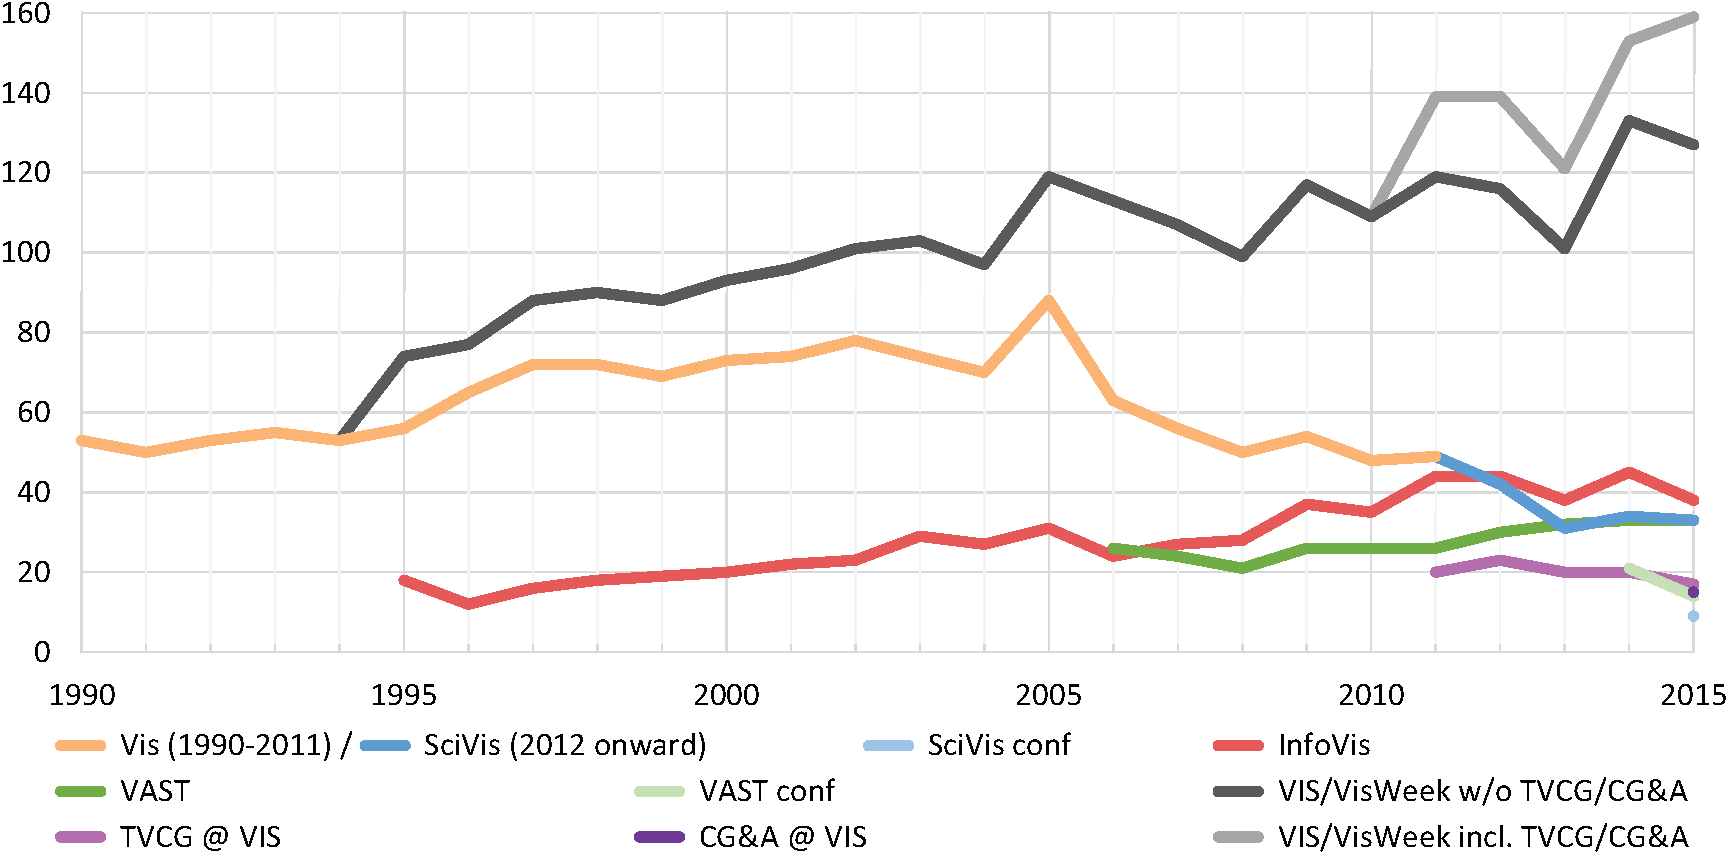
\includegraphics[width=\columnwidth]{paper-count-w-2015-new}
 \caption{A visualization of the 1990--2015 data from \autoref{tab:vis_papers}. The image is from \cite{Isenberg:2017:VMC} and is in the public domain.}
 \label{fig:sample}
\end{figure}

\subsubsection{Ejector Seat Reservation}

Duis autem~\cite{Lorensen:1987:MCA}\footnote{The algorithm behind
Marching Cubes \cite{Lorensen:1987:MCA} had already been
described by Wyvill et al. \cite{Wyvill:1986:DSS} a year
earlier.} vel eum iriure dolor in hendrerit
in vulputate velit esse molestie consequat,\footnote{Footnotes
appear at the bottom of the column.} vel illum dolore eu
feugiat nulla facilisis at vero eros et accumsan et iusto odio
dignissim qui blandit praesent luptatum zzril delenit augue duis
dolore te feugait nulla facilisi. Lorem ipsum dolor sit amet,
consectetuer adipiscing elit, sed diam nonummy nibh euismod tincidunt
ut laoreet dolore magna aliquam erat volutpat.


\paragraph{Confirmed Ejector Seat Reservation}

Ut wisi enim ad minim veniam, quis nostrud exerci tation ullamcorper
suscipit lobortis nisl ut aliquip ex ea commodo
consequat~\cite{Nielson:1991:TAD}. Duis autem vel eum iriure dolor in
hendrerit in vulputate velit esse molestie consequat, vel illum dolore
eu feugiat nulla facilisis at vero eros et accumsan et iusto odio
dignissim qui blandit praesent luptatum zzril delenit augue duis
dolore te feugait nulla facilisi.

\paragraph{Rejected Ejector Seat Reservation}

Ut wisi enim ad minim veniam, quis nostrud exerci tation ullamcorper
suscipit lobortis nisl ut aliquip ex ea commodo consequat. Duis autem
vel eum iriure dolor in hendrerit in vulputate velit esse molestie


\section{Conclusion}

Lorem ipsum dolor sit amet, consetetur sadipscing elitr, sed diam
nonumy eirmod tempor invidunt ut labore et dolore magna aliquyam erat,
sed diam voluptua. At vero eos et accusam et justo duo dolores et ea
rebum. Stet clita kasd gubergren, no sea takimata sanctus est Lorem
ipsum dolor sit amet. Lorem ipsum dolor sit amet, consetetur
sadipscing elitr, sed diam nonumy eirmod tempor invidunt ut labore et
dolore magna aliquyam erat, sed diam voluptua. At vero eos et accusam
et justo duo dolores et ea rebum. Stet clita kasd gubergren, no sea
takimata sanctus est Lorem ipsum dolor sit amet. Lorem ipsum dolor sit
amet, consetetur sadipscing elitr, sed diam nonumy eirmod tempor
invidunt ut labore et dolore magna aliquyam erat, sed diam
voluptua. At vero eos et accusam et justo duo dolores et ea
rebum.


%% if specified like this the section will be committed in review mode
\acknowledgments{
The authors wish to thank A, B, and C. This work was supported in part by
a grant from XYZ.}

%\bibliographystyle{abbrv}
\bibliographystyle{abbrv-doi}
%\bibliographystyle{abbrv-doi-narrow}
%\bibliographystyle{abbrv-doi-hyperref}
%\bibliographystyle{abbrv-doi-hyperref-narrow}

\bibliography{template}
\end{document}
